\section{Introduction}
\subsection{Motivation}
\begin{frame}[<+->]
	\frametitle{Motivation}
	We want to apply and refine results from real complexity theory to develop 
efficient numerical algorithms with the following properties:
\begin{itemize}[<+->]
	\item full specification
	\item sound semantics
	\item correctness
	\item closure under composition
\end{itemize}

\end{frame}
\begin{frame}
	\frametitle{Algorithm Engineering}
	\centering
	\includegraphics[width=0.7\textwidth]{approach.png}
\end{frame}
\begin{frame}[<+->]
\frametitle{iRRAM}
\begin{itemize}[<+->]
\item iRRAM is a C++ framework for exact real computations
\item Ordinary C++ is extended by datatype REAL for computing with real numbers
\item Usual arithmetic operations are implemented for REAL
\item Other functions like abs, power, root, modulo, exp, log, sin, cos are also available
\end{itemize}
\end{frame}
\begin{frame}
  \frametitle{\irram: Real Number Representation}
  \centering
    \begin{tikzpicture}[remember picture, overlay]
     \node[font=\huge] at (0,0) {$x \in [\textcolor{green}{d}-\textcolor{red}{e},\textcolor{green}{d}+\textcolor{red}{e}]$};
     \draw<2-> [->, line width=3pt,color=green] (-1,0.4) -- (-1,2);
     \node<2->[color=green,font=\large] at (-1,2.2) {Multiple precision floating point number};
     \draw<3-> [->, line width=3pt,color=red] (2.4,-0.4) -- (2.4,-2);
     \node<3->[color=red,font=\large] at (2.4,-2.2) {$e = z \cdot 2^p$ (p,z \code{long})};
    \end{tikzpicture}
\end{frame}

\begin{frame}[<+->][fragile]
\frametitle{Example: \irram}
\begin{example}
\begin{lstlisting}
REAL series(int n){
  return power(REAL(2), -n);
}
REAL xinv_approx(long p, REAL& x){
  int N=-2*p+3;
  REAL ans = 0.0;
  for(int i=0; i<=N; i++)
    ans += series(i)*power(x,i);
  return ans;
}
REAL xinv(REAL& x) { return limit(xinv_approx, x);}
\end{lstlisting}
\end{example}
\end{frame}
